\def\bmsBoardWidth{5}
\def\bmsBoardHeight{1.7}

\def\bmsBvlX{0.3}
\def\bmsBvlY{0.3}

\def\bmsIcWidth{0.75}
\def\bmsIcHeight{0.7}

\def\bmsSolPadWidth{0.25}
\def\bmsSolPadHeight{0.2}

\ctikzsubcircuitdef{spicbms} {
    bp, bn, b1, b2, pp, pn%
} {
    coordinate (#1-origin)
    ++({\bmsBoardWidth/2},{-\bmsBoardHeight/2})
    node [inner sep = 0pt, anchor = center] {
        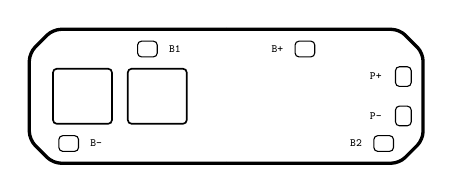
\begin{tikzpicture}
            \draw
            (0,0) coordinate (origin)
            (origin) ++({\bmsBoardWidth/2},0)
            coordinate (mid)
            ;
            %% board
            \draw [very thick, rounded corners = 1mm]
            (mid) -- ++({-(\bmsBoardWidth/2)+\bmsBvlX},0)
            -- ++(-\bmsBvlX,-\bmsBvlY)
            -- ++(0,{-\bmsBoardHeight+(2*\bmsBvlY)})
            -- ++(\bmsBvlX,-\bmsBvlY)
            -- ++({(\bmsBoardWidth/2)-\bmsBvlX},0)
            ;
            \draw [very thick, rounded corners = 1mm]
            (mid) -- ++({(\bmsBoardWidth/2)-\bmsBvlX},0)
            -- ++(\bmsBvlX,-\bmsBvlY)
            -- ++(0,{-\bmsBoardHeight+(2*\bmsBvlY)})
            -- ++(-\bmsBvlX,-\bmsBvlY)
            -- ++({-(\bmsBoardWidth/2)+\bmsBvlX},0)
            ;
            %% drawing ics
            \draw [semithick, rounded corners = 0.5mm]
            (origin) ++(\bmsBvlX,-0.5)
            rectangle ++(\bmsIcWidth,-\bmsIcHeight)
            (origin) ++({\bmsBvlX+\bmsIcWidth+0.2},-0.5)
            rectangle ++(\bmsIcWidth,-\bmsIcHeight)
            ;
            %% battery solder pads
            \draw [rounded corners = 0.5mm]
            (mid) ++({\bmsBoardWidth/5},-0.25)
            node [left = 5pt, font = \tiny, scale = 0.8] {\texttt{B+}}
            ++({-\bmsSolPadWidth/2},{\bmsSolPadHeight/2})
            rectangle ++(\bmsSolPadWidth,-\bmsSolPadHeight)
            %%
            (mid) ++({-\bmsBoardWidth/5},-0.25)
            node [right = 5pt, font = \tiny, scale = 0.8] {\texttt{B1}}
            ++({-\bmsSolPadWidth/2},{\bmsSolPadHeight/2})
            rectangle ++(\bmsSolPadWidth,-\bmsSolPadHeight)
            %%
            (mid) ++({\bmsBoardWidth/5*2},{-\bmsBoardHeight+0.25})
            node [left = 5pt, font = \tiny, scale = 0.8] {\texttt{B2}}
            ++({-\bmsSolPadWidth/2},{\bmsSolPadHeight/2})
            rectangle ++(\bmsSolPadWidth,-\bmsSolPadHeight)
            %%
            (mid) ++({-\bmsBoardWidth/5*2},{-\bmsBoardHeight+0.25})
            node [right = 5pt, font = \tiny, scale = 0.8] {\texttt{B-}}
            ++({-\bmsSolPadWidth/2},{\bmsSolPadHeight/2})
            rectangle ++(\bmsSolPadWidth,-\bmsSolPadHeight)
            %%
            ;
            %% input
            \draw [rounded corners = 0.5mm]
            (origin) ++({\bmsBoardWidth},{-\bmsBoardHeight/2})
            ++(-0.25,0.25)
            node [left = 5pt, font = \tiny, scale = 0.8] {\texttt{P+}}
            ++({-\bmsSolPadHeight/2},{\bmsSolPadWidth/2})
            rectangle ++(\bmsSolPadHeight,-\bmsSolPadWidth)
            %%
            (origin) ++({\bmsBoardWidth},{-\bmsBoardHeight/2})
            ++(-0.25,-0.25)
            node [left = 5pt, font = \tiny, scale = 0.8] {\texttt{P-}}
            ++({-\bmsSolPadHeight/2},{\bmsSolPadWidth/2})
            rectangle ++(\bmsSolPadHeight,-\bmsSolPadWidth)
            ;
        \end{tikzpicture}
    }
    %% marking solder pads
    (#1-origin) ++({\bmsBoardWidth/2},0) coordinate (#1-mid)
    %%
    (#1-mid) ++({\bmsBoardWidth/5},0)
    coordinate (#1-bp)
    %%
    (#1-mid) ++({-\bmsBoardWidth/5},0)
    coordinate (#1-b1)
    %%
    (#1-mid) ++({\bmsBoardWidth/5*2},-\bmsBoardHeight)
    coordinate (#1-b2)
    %%
    (#1-mid) ++({-\bmsBoardWidth/5*2},-\bmsBoardHeight)
    coordinate (#1-bn)
    %% marking +ve and -ve terminals
    (#1-origin) ++({\bmsBoardWidth},{-\bmsBoardHeight/2})
    ++(0,0.25) coordinate (#1-pp)
    %%
    (#1-origin) ++({\bmsBoardWidth},{-\bmsBoardHeight/2})
    ++(0,-0.25) coordinate (#1-pn)
}

\ctikzsubcircuitactivate{spicbms}
